\documentclass[a4paper,12pt, oneside]{book}

% \usepackage{fullpage}
\usepackage[italian]{babel}
\usepackage[utf8]{inputenc}
\usepackage{amssymb}
\usepackage{amsthm}
\usepackage{graphics}
\usepackage{amsfonts}
\usepackage{listings}
\usepackage{amsmath}
\usepackage{amstext}
\usepackage{engrec}
\usepackage{rotating}
\usepackage{verbatim}
\usepackage[safe,extra]{tipa}
\usepackage{showkeys}
\usepackage{multirow}
\usepackage{hyperref}
\usepackage{microtype}
\usepackage{enumerate}
\usepackage{braket}
\usepackage{marginnote}
\usepackage{pgfplots}
\usepackage{cancel}
\usepackage{polynom}
\usepackage{booktabs}
\usepackage{enumitem}
\usepackage{framed}
\usepackage{pdfpages}
\usepackage{pgfplots}
\usepackage{algorithm}
%\usepackage{algpseudocode}
\usepackage[cache=false]{minted}
\usepackage{mathtools}
\usepackage{algpseudocode}
\usepackage{tikz}\usetikzlibrary{er}\tikzset{multi  attribute /.style={attribute ,double  distance =1.5pt}}\tikzset{derived  attribute /.style={attribute ,dashed}}\tikzset{total /.style={double  distance =1.5pt}}\tikzset{every  entity /.style={draw=orange , fill=orange!20}}\tikzset{every  attribute /.style={draw=MediumPurple1, fill=MediumPurple1!20}}\tikzset{every  relationship /.style={draw=Chartreuse2, fill=Chartreuse2!20}}\newcommand{\key}[1]{\underline{#1}}


\usepackage{fancyhdr}
\pagestyle{fancy}
\fancyhead[LE,RO]{\slshape \rightmark}
\fancyhead[LO,RE]{\slshape \leftmark}
\fancyfoot[C]{\thepage}



\title{Analisi e Progetto di Algoritmi}
\author{UniShare\\\\Davide Cozzi\\\href{https://t.me/dlcgold}{@dlcgold}\\\\Gabriele De Rosa\\\href{https://t.me/derogab}{@derogab} \\\\Federica Di Lauro\\\href{https://t.me/f_dila}{@f\textunderscore dila}}
\date{}

\pgfplotsset{compat=1.13}
\begin{document}
\maketitle

\definecolor{shadecolor}{gray}{0.80}
\setlist{leftmargin = 2cm}
\newtheorem{teorema}{Teorema}
\newtheorem{definizione}{Definizione}
\newtheorem{esempio}{Esempio}
\newtheorem{corollario}{Corollario}
\newtheorem{lemma}{Lemma}
\newtheorem{osservazione}{Osservazione}
\newtheorem{nota}{Nota}
\newtheorem{esercizio}{Esercizio}
\algdef{SE}[DOWHILE]{Do}{doWhile}{\algorithmicdo}[1]{\algorithmicwhile\ #1}
\tableofcontents
\renewcommand{\chaptermark}[1]{%
  \markboth{\chaptername
    \ \thechapter.\ #1}{}}
\renewcommand{\sectionmark}[1]{\markright{\thesection.\ #1}}
\chapter{Introduzione}
\textbf{Questi appunti sono presi a lezione. Per quanto sia stata fatta una revisione è altamente probabile (praticamente certo) che possano contenere errori, sia di stampa che di vero e proprio contenuto. Per eventuali proposte di correzione effettuare una pull request. Link: } \url{https://github.com/dlcgold/Appunti}.\\
\textbf{Grazie mille e buono studio!}
\\
\begin{comment}

  \begin{algorithm}
    \If {$i \gets 1$}
    \State $test$
    \Else
    \State $bho$
    \EndIf
    \While {$test$}
    \State $cose$
    \EndWhile
    \For {$cose...$}
    \State $altre cose$
    \EndFor

    \Function{Increment}{$a$}
    \State $a \gets a+1$
    \State \Return $a$
    \EndFunction
  \end{algorithm}

  \begin{algorithm}
    \Do
    \State ciao
    \doWhile {$ciao$}
  \end{algorithm}
\end{comment}
\chapter{Introduzione al corso}
\section{Argomenti}
Si hanno diversi tipi di problemi:
\begin{itemize}
  \item \textbf{problemi di ottimo} dove si cercano singole soluzioni
  efficienti (massimi o minimi) tra molte soluzioni possibili. Si
  usa anche la \textbf{programmazione greedy}, dove si sceglie in base
  ai costi locali per ottenere massimi e minimi senza però guardare i
  costi complessivi.   
  \item \textbf{problemi non risolubili in tempi accettabili}, per i
  quali si usa la \textbf{programmazione dinamica}, che cerca di
  individuare sotto-strutture ottime per risolvere il problema,
  cercando la soluzione migliore memorizzando le altre soluzioni e
  utilizzandole. Si cerca comunque la soluzione meno dispendiosa in
  termini di tempo.
  \item \textbf{problemi NP-completi}, ovvero problemi per cui non si
  può trovare un algoritmo o non si può trovare un algoritmo con una
  complessità asintotica polinomiale. Si useranno anche tecniche non
  deterministiche. Si cercherà di studiare uno dei 10 problemi più
  difficili della matematica: $P\subseteq NP$?
\end{itemize}
Studieremo poi i grafi non pesati con gli algoritmi \textit{BFS}
(per cercare in ampiezza) e \textit{DFS} (per cercare in
profondità). Studieremo anche i grafi pesati con problemi di cammino
minimo.\\
\section{Ripasso Algoritmi 1}
Innazitutto due algoritmi con lo stesso scopo si possono confrontare
in base a tempo e spazio, scegliendo anche in base alle esigenze
hardware. Per lo spazio si calcola quanto spazio viene richiesto da
variabili e strutture dati, soprattutto queste ultime che dipendono
dalla dimensione dell'input. Per quanto riguarda il tempo si usano le
tecniche di conto soprattutto basate sui cicli e, in generale, su
tutte operazioni da effettuare. Il tempo si basa sull'input $n$ e si
indica con $T(n)$ e si esprime in forma asintotica, interessandoci
quindi unicamente all'ordine di grandezza. Si hanno il caso peggiore,
indicato con l'O-grande e quello migliore indicato con l'o-piccolo
a seconda di $n$.\\
Si ricorda poi la tecnica della ricorsione con algoritmi che si
muovono su se stessi mediante dei ``passi'' arrivando ad un caso base
di uscita. Per calcolare i tempi di un algoritmo ricorsivo si ha
$T(n)=F(n)+T(n-1)$ con $F$ che rappresenta le istruzioni delle
subroutines. Questa equazione di ricorrenza non è facilmente
calcolabile ma può essere espansa muovendosi sui passi fino a che non
si arriva a qualcosa di calcolabile grazie al caso 0, questo è il
metodo iterativo (anche se si ha anche il metodo per
sostituzione). Per gli algoritmi ricorsivi si hanno anche i divide et
impera (dove il problema P è diviso in sottoproblemi risolti
separatemente, con la divide, e poi combinati alla fine, con la
combina) dove i tempi non sono sempre calcolabili ma se lo sono
si usa il metodo dell'esperto (studiando le tre possibili casistiche).
\begin{shaded}
  \subsection{Equazioni di Ricorrenza}
  Le equazioni di ricorrenza hanno solitamente la seguente forma:
  $$\begin{cases}
    T(n)=T(n-1)+f(n) \\
    T(1)=\Theta(1)
  \end{cases}$$
  Esistono tre metodi per risolvere le equazioni di ricorrenza:
  \begin{itemize}
    \item Iterativo (detto anche Albero di ricorsione)
    \item Sostituzione
    \item Esperto (detto anche Principale)
  \end{itemize}
  \subsubsection{Metodo Iterativo}
  Si può usare sia per algoritmi ricorsivi e per Divide et Impera.
  Ad ogni passo si prende il valore a destra dell'uguaglianza e
  lo si sostituisce, arrivando, dopo $k$ passi ad una formula
  generale. Sempre $k$ ci darà il caso base. Posso rappresentare
  questo  metodo con l'albero delle chiamate ricorsive,
  guardando quanto è alto l'albero e quanto impiega ad ogni livello
  \begin{esempio}
    Calcolo i tempi di:
    $$\begin{cases}
      T(N)=T(n-1)+8 \\
      T(1)=6
    \end{cases}$$
    procedo nella seguente maniera:
    $$T(n)=T(n-1)+8=[T(n-2)+8]+8=T(n-2)+2\cdot 8$$
    $$=[T(n-3)+8]+2\cdot 8= T(n-3)+3\cdot 8$$
    $$=[T(n-4)+8]+3\cdot 8=T(n-4)+4\cdot 8$$
    $$=T(n-k)+k\cdot 8$$
    per $k=n-1$ si ha:
    $$T[n-(n-1)]+(n-1)\cdot 8=T(1)+(n-1)\cdot 8=6+(n-1)\cdot 8=\Theta(n)$$
  \end{esempio}
  \textit{Altri esempi su sito e appunti di Chiodini}
  \subsubsection{Metodo per Sostituzione}
  Si ipotizza un tempo di calcolo (si possono usare gli
  asintotici con $O$ e $\Omega$ lo si dimostra per induzione
  \begin{esempio}
    $$\begin{cases}
      T(n)=2\cdot T\left(\frac{n}{\floor{2}}\right)+n & n>1 \\
      T(1)                                            & n=1
    \end{cases}
    $$
    Ipotizzo $O(n\cdot \log n)$ e dimostro per induzione:
    $$T(n)=O(n\cdot \log n)\leq c\cdot n\cdot \log n$$
    Serve una dimostrazione forte:
    ipotizzo $T(m)$ vera per $1\leq m\leq n-1$ quindi si ha:
    $$T(n)=2\cdot T\left(\frac{n}{\floor{2}}\right)+n\leq 2\cdot \left[c\cdot \frac{n}{\floor{2}}\cdot \log \frac{n}{\floor{2}}\right]+n$$
    $$=c\cdot n\cdot \log \frac{n}{2}+n=c\cdot n\cdot (\log_2 n-\log_2 2)+n$$
    $$=c\cdot n\cdot \log_2 n-c\cdot n+n\leq c\cdot n\cdot \log n \mbox{ se } c\geq 1$$
    \newpage
    Analizzo ora il caso base:\\
    $T(1)=1$ quindi voglio $1\leq c\cdot \log_2 1$ ovvero $1\leq c\cdot 0$ ovvero mai.
    testo fino a che non trovo $T(3)=2\cdot T(1)+3=29+3=5$ che mi va bene, infatti $5\leq c\cdot 3\cdot \log_2 3$
  \end{esempio}
  \subsubsection{Metodo dell'Esperto}
  Posso usare questo metodo solo nel caso di un'equazione di ricorrenza di questo tipo:
  $$\begin{cases}
    T(n)=a\cdot T\left(\frac{n}{b}\right) +f(n) \\
    T(1)=\Theta(1)
  \end{cases}$$
  dove:
  \begin{itemize}
    \item $a\cdot T\left(\frac{n}{b}\right)$ è l'Impera ed è $\sim n^{\log_b a}$
    \item $f(n)$ è il divide e il combina (ovvero la parte iterativa)
  \end{itemize}
  Si definiscono tre casi:
  \begin{itemize}
    \item \textbf{caso 1:} $n^{\log_b a}>f(n)$ quindi $T(n)\sim n^{\log_b a}$. Si hanno le seguenti condizioni necessarie: $f(n)=O(n^{log_b a -\epsilon})$ ( con $\epsilon>0$) e quindi $T(n)=\Theta(n^{log_b a -\epsilon})$
    \item \textbf{caso 2:} $n^{\log_b a}\cong f(n)$ quindi $T(n)\sim f(n)\cdot \log n$. Si hanno le seguenti condizioni necessarie $f(n)=\Theta(n^{\log_b a})$ e quindi $T(n)=\Theta(n^{\log_b a})$
    \item \textbf{caso 3:} $n^{\log_b a}< f(n)$ quindi $T(n)\sim f(n)$. Si hanno le seguenti condizioni necessarie: $f(n)=\Omega(n^{\log_b a +\epsilon})$ (con $\epsilon>0$) e $a\cdot f\left(\frac{n}{b}
    \right)\leq k\cdot f(n)$ (con $k<1$) quindi $T(n)=\Theta(f(n))$
  \end{itemize}

  \begin{esempio}
    Risolvo:
    $$T(n)=9\cdot T\left(\frac{n}{3}\right)+n$$
    Si ha: $f(n)=n$, $a=9$ e $b=3$.\\
    Ho che $n^{\log_3 9}=n^2$ quindi ho il primo caso:\\
    $f(n)=O(n^{\log_b a -\epsilon})=O(n^{2-\epsilon})$
    Posso dire che $\exists \epsilon:\, O(n^{2-\epsilon})=n$?\\
    Si $\forall \epsilon<1$, per esempio $\epsilon=\frac{1}{2}$. Quindi il Metodo dell'esperto è applicabile (nel primo caso) e si ha quindi $T(n)=\Theta(n)$
  \end{esempio}
  \newpage
  \begin{esempio}
    Si può analizzare meglio il MergeSort:
    $$T(n)\cong 2\cdot T\left(\frac{n}{2}\right)+\Theta(n)$$
    Si ha: $f(n)=\Theta(n)$ e $n^{\log_b a}=n^{\log_2 2 }=n$\\
    Posso applicare il Metodo dell'esperto nel secondo caso avendo così: $$T(n)=\Theta(n\cdot \log n)$$
  \end{esempio}
  \begin{esempio}
    $$T(n)=3\cdot T\left(\frac{n}{4}\right)+n\cdot \log n$$
    Si ha: $f(n)=n\cdot \log n$ e $n^{\log_b a}=n^{\log_4 3}$ e siamo nel terzo caso:
    $$f(n)=\Omega(n^{\log_4 3+\epsilon}$$
    se pongo $\epsilon=1-\log_4 3$ ottengo $n$.
    Il terzo caso richiede una doppia verifica:
    $$3\cdot \frac{n}{4}\cdot\log \frac{n}{4}\leq k\cdot n\log n$$
    che vale per $k=\frac{3}{4}$ infatti si ha:
    $$\frac{3}{4}\cdot n\cdot\log \frac{n}{4}\leq \frac{3}{4} \cdot n\cdot \log n$$
    Si hanno quindi entrambi i requisiti e si può asserire che $T(n)=\Theta(n\cdot\log n)$
  \end{esempio}
  \begin{esempio}
    Calcolo i tempi di:
    $$T(n)=2\cdot T\left(\frac{n}{2}\right)+n\cdot\log n$$
    Si ha: $n^{\log_b a }=n^{\log_2 2 }=n$ e $f(n)=n\cdot\log n$.
    Provo a procedere col terzo caso, dimostrando che: $$n\cdot\log n=\Omega(n^{\log_b a +\epsilon})=\Omega(n^{1+\epsilon})=\Omega(n\cdot n^\epsilon)$$
    Ma tale $\epsilon$ non esiste in quanto $n^\epsilon>\log n$ infatti:
    $$\lim_{n\rightarrow \infty}\frac{n\cdot\log n}{n\cdot n^\epsilon}=0,\,\,\, \forall\, \epsilon>0$$
    Bisogna quindi applicare un altro metodo per risolvere l'equazione di ricorrenza
  \end{esempio}
  \begin{esempio}
    Calcolo la seguente equazione di ricorrenza:
    \[\
      \begin{cases}
        T(n)=1 & n=1\\
        T(n)= 2\cdot T(\frac{n}{2})+1 & n>1
      \end{cases}
    \]
    Quindi avrò un albero binario di soli 1 di profonfità $2^k$
    Quindi $T(n)=\sum_{i=0}^k2^i=2^{k+1}-1$ con $k=\log n$ in quanto si avranno
    in totale $n=2^k=2\cdot2^k-1$. Quindi ottengo $2n-1$ quindi
    avrò $\Theta(n)$.
  \end{esempio}
\end{shaded}
Abbiamo poi visto alcune strutture dati: \textit{array, list, stack, queue,
  tree (e binary-tree) e heap}. 
\chapter{Programmazione Dinamica}
Partiamo dall'algoritmo che calcola la lista di Fibonacci:
\begin{shaded}
  \begin{algorithmic}
    \Function{$FIB$}{$n$}
    \If {$n=1$}
    \State $return\,\,n$
    \Else
    \State $return\,\,FIB(n-1)+FIB(n-2)$
    \EndIf
    \EndFunction
  \end{algorithmic}
\end{shaded}
\\
Si vede che non sappiamo calcolarne la compplessità, che non è
polinomiale ma magari esponenziale o addirittura fattoriale.\\
Sia $T(n)$ il costo della chiamata alla funzione. Se $n=0$ o $n=1$ ho
$T(n)=1$. Andando avanti avrò $T(n)=1+T(n-1)+T(n-2)$ che non è
risolvibile con le tecniche che conosciamo. Vediamo come risolverla:
riscriviamo l'equazione non omogenea:
\[T(n)-T(n-1)-T(n-2)=1\]
e facciamo una piccola approssimazione:
\[T(n)-T(n-1)-T(n-2)=0\]
ottenendo un'equazione lineare omogenea a cui sommerò qualcosa per
ottenre il risultato della non omogenea. Quindi risolvo l'omogenea
ipotizzando un valore per $T(n)$, per esempio $T(n)=r^n$, e
testiamolo, diventa:
\[r^n-r^{n-1}-r^{n-2}=0\]
moltiplico da entrambe le parti per $r^2$ perché posso:
\[r^2\cdot r^n-r\cdot r^n-r^n=0\]
\[r^2-r-1=0\]
che è un'equazione di secondo grado con soluzioni
$r=\frac{1\pm\sqrt{5}}{2}$
Quindi
\[T(n)-T(n-1)-T(n-2)=0\]
ha due soluzioni:
\[C_1\left(\frac{1+\sqrt{5}}{2}\right)^{n}\]
\[C_2\left(\frac{1-\sqrt{5}}{2}\right)^{n}\]
quindi:
\[T_0(n)=C_1\left(\frac{1+\sqrt{5}}{2}\right)^{n} + C_2
  \left(\frac{1-\sqrt{5}}{2}\right)^{n}\]
Ora cerco la soluzione particolare, sostituisco in:
\[T(n)-T(n-1)-T(n-2)=1\]
Tutte le $T(\cdot)$ con $k$ ottenendo $k-k-k=1\to k = -1$.\\
Quindi la soluzione finale è:
\[T(n)=C_1\left(\frac{1+\sqrt{5}}{2}\right)^{n} +C_2
  \left(\frac{1-\sqrt{5}}{2}\right)^{n}-1=\Theta\left(\left(\frac{1+\sqrt{5}}{2}\right)^{n}\right)\]
\textit{che è la sezione aurea}\\
Miglioriamo l'algoritmo introducendo un array di $n$ celle $F$,
inizializzarlo
\begin{shaded}
  \begin{algorithmic}
    \State $F[1\ldots n]$
    \For {$i\gets1\,\,to\,\, n$}
    \State $F[i]\gets empty$
    \EndFor
  \end{algorithmic}
\end{shaded}
e procedere con la ricorsione con annotazione, che scrive i vari step
su un array (sprecando quindi memoria) e modificando fibonacci per
ottenre la versione con annotazione:
\begin{shaded}
  \begin{algorithmic}
    \Function{$FIBANN$}{$n$}
    \If {$f[i]== empty$}
    \If {$n\leq 1$}
    \State $F[n]\gets n$
    \Else
    \State $F[n]=FIBANN(n-1)+FIBANN(n-2)$
    \EndIf
    \State $return\,\,F[n]$
    \EndIf
    \EndFunction
  \end{algorithmic}
\end{shaded}
Quindi se si richiede qualcosa di già usato lo si ritorna prendendolo
dall'array. Questo è esponenziale\\
Iterativamente sarebbe:
\begin{shaded}
  \begin{algorithmic}
    \Function{$FIBIT$}{$n$}
    \State $F[0] \gets 0$
    \State $F[1] \gets 1$
    \For {$i\gets 2\,\,to\,\,n$}
    \State $F[i] \gets F[i-1]+F[i-2]$
    \EndFor
    \State $return\,\,F[n]$
    \EndFunction
  \end{algorithmic}
\end{shaded}
questo è polinomiale
\subsubsection{Un Nuovo Problema}
Abbiamo una serie di task che possono essere svolte con un certo costo
$v_i$, che partono in tempi diversi e non possono essere svolte
contemporaneamente:
\begin{center}
  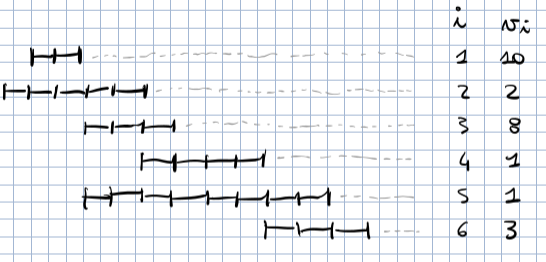
\includegraphics[scale = 0.7]{img/ta.png}
\end{center}
Per ogni attività si ha quindi un $s_i$, tempo di inizio, un $f_i$,
tempo di fine, e un $v_i$, il costo, con $i\ldots n$ che indica
l'attività. Definiamo $A\subseteq\{1,\ldots, n\}$ come l'insieme che
contiene attività mutualmente compatibili sse:
\[\forall i,j\in A\,\, [s_i,f_i)\cap [s_j,f_j)\neq \emptyset\]
definiamo anche $comp(A)$:
\[
  \begin{cases}
    $true$ & \mbox{ se mutualmente compatibili}\\
    $false$ & \mbox{ altrimenti}
  \end{cases}
\]
che verifica se dei task sono mutualmente compatibili.\\

Inoltre $V(A)=\sum_{i\in A}v_i$ per vedere il costo totale di una
serie di task, con:
\[P(\{1,\ldots, n\})\to \{true,\,false\}\]
\[V:P(\{1,\ldots, n\})\to \mathbb{R}\]
Quindi la soluzione sarà un insieme di task tale che:
\[S\subseteq \{1,\ldots, n\} \to
  comp(S)=true,\,\, V(S)=\max\{v(A)\}\]
Definiamo in maniera formale:
l'instanza è una $n\in\mathbb{N}$ e $X_n\in\{1,\ldots,n\}$. Ad ogni
attività $i\in X_n$ ci sono associate il tempo di inizio $s_i$, di fine $f_i$
e il valore $v_i$.\\
La soluzione è un sottoinsieme $S\subseteq X_N$ di attività
compatibili secondo la funzione \textit{comp} e tale che
$v(S)=\max_{A\subseteq X_n,\, comp(A)=TRUE}\{v(A)\}$.
La soluzione basata sulla forza bruta (calcolo tutte le combinazioni)
è $\Omega(2^n)$ nel caso migliore; non va bene.\\
Usiamo quindi la programmazione dinamica devo però prima cercare la
soluzione in termini ricorsivi, cercando i sottoproblemi. La struttura
da ``far calare'' è $X_n$ a step di $n-1$ lavorando quindi su
$S_{n-1}\subseteq X_{n-1}$ tale che valga quanto sopra.\\ Il
sottoprobelma i-esimo sarà $X_i=\{1,\ldots i\}$ con $S_i\subseteq X_i$
con le condizioni di sopra.\\
Il sottoproblema con $i=1$ avrà $X_1=\{1\}$ fatto solo dalla prima
attività e quindi avrò $S_1 = \{1\}$ e quindi $v(S_1)= v_1$, ovvero
$10$ nel nostro caso.\\
Inoltre se $i=0$ avrò l'insieme vuoto che ha valore 0. \\
Quindi $S_1 = \{1\}$, con $V(S_1)=1$, e $S_0 = \emptyset$, con
$v(s_0)=0$ e questi potrebbero essere i miei casi base. \\
Ragioniamo su 6, se 6 è soluzione allora sarà insieme alla soluzione
delle altre attività compatibili, ovvero quella di 4 essendo la prima
compatibile in ordine, o meglio $s_6 = \{6\}\cup S_4$. Per la 5 sarà
1, per la 4 sarà 2, per la 3 sarà 1 e per la 2 non sarà nessuna, come per
1, e quindi sarà 0. Ho appena definito $p(i) =\max\{j|\, j< i,\,
\mbox{ j compatibile con i}\}$ assumendo che $\max \emptyset = 0$,
quindi l'attività con indice maggiore compatibile precedente a quella
in studio.\\
\textbf{Questo schema funziona per attività ordinate sull'ordine di
  fine}.\\

Quindi:
\[
  S_i=\begin{cases}
    \{i\}\cup S_{p(i)} & \mbox{se }i\in S_i\\
    S_{i-1} & \mbox{se } i\not\in S_i
  \end{cases}
\]
e:
\[
  v(S_i)=\begin{cases}
    v_i+v(S_{p(i)})\\
    v(S_{i-1})
  \end{cases}
\]
Il modo di procedere consiste nel valcolare i valori e aggiornare il
massimo:
\[v(S_i)=\max\{v_i+v(S_{p(i)}),\, v(s_{i-1})\},\,i>0\]
sapendo $v(S_1)=1$ e $v(s_0) = 0$.\\
Ma in realtà $v(S_1)=1$ è ricavabile da $v(S_0)$ con la formula quindi
avremo solo un caso base: $v(S_0)=0,\,i=0$.\\
Quindi abbiamo trovato la ricorrenza, considerando anche che:
\[
  S_i=\begin{cases}
    \{i\}\cup S_{p(i)} & \mbox{se }v_i+v(S_{p(i)}) \geq v(S_{i-1})\\
    S_{i-1} & \mbox{se } v_i+v(S_{p(i)}) < v(S_{i-1}
  \end{cases}
\]
\newpage
Quindi ottengo l'algoritmo ricorsivo per calcolare i vari $v_i$:
\begin{shaded}
  \begin{algorithmic}
    \Function{$R\_OPT$}{$i$}
    \If{$i == 0$}
    \State \textbf{return} $0$
    \Else
    \State \textbf{return} $\max(v_i+R\_OPT(p[i]), R\_OPT(i-1))$
    \EndIf
    \EndFunction
  \end{algorithmic}  
\end{shaded}
Ma è ingestibile dal punto di vista della complessità. Utilizzo quindi
un vettore $M[0..n]$, introducendo la programmazione dinamica,
dove in $M[i]$ memorizzo il valore della soluzione del problema di
taglia $i$, ovvero $v(S_i)$.\\
Facciamo quindi la ricorsione con l'annotazione:
\begin{shaded}
  \begin{algorithmic}
    \For {$j\gets 0$ \textbf{to} $n$}
    \State $M[j]\gets \mbox{\textit{empty}}$
    \EndFor
    
    \Function{$AR\_OPT$}{$i$}
    \If{$M[i] == \mbox{\textit{empty}}$}
    \If {$i==0$}
    \State $M[i]\gets 0$
    \Else
    \State $M[i]\gets\max(v_i+AR\_OPT(p[i]), AR\_OPT(i-1))$
    \EndIf
    \EndIf
    \State \textbf{return} $M[i]$
    \EndFunction
  \end{algorithmic}  
\end{shaded}
che resta una tecnica \textit{top-down}. Ma solitamente si lavora
\textit{bottom-up} nella programmazione dinamica. Quindi non abbiamo
di caricare l'array e non abbiamo bisogno di if/else:
\begin{shaded}
  \begin{algorithmic}
    \Function{$PD\_OPT$}{$i$}
    \State $M[0]\gets 0$
    \For {$j\gets 1$ \textbf{to} $i$}
    \State $M[j]\gets\max(v_j+M[P[j]], M[J-1])$
    \EndFor
    \State \textbf{return} $M[i]$
    \EndFunction
  \end{algorithmic}  
\end{shaded}
\textbf{ovviamente prima di tutto ho il caricamento di p[i], come è
  stato descritto sopra}.\\
Ora si ha una complessità pari a $\Theta(n)$ per quest'ultimo
algortimo, che calcola $v(S_i)$ ma bisogna sommare $\Theta(n\log n)$,
in quanto bisogna ordinare le attività sul tempo di fine.\\
Ora devo capire cos'è $S_i$, uso il \textbf{weighted interval
  scheduling} per stamparlo (usando l'array $M$), usando un algoritmo
ricorsivo che non ripete cose già usare, un algoritmo ricorsivo in
coda che quindi è comodo ed efficiente da lasciare ricorsivo:
\begin{shaded}
  \begin{algorithmic}
    \Function{$WIS\_PRINT$}{$i$}
    \If {$i\neq 0$}
    \If {$v_i+M[p(i)] \geq M[i-1]$}
    \State $print(i)$
    \State $WIS\_PRINT(p(i))$
    \Else
    \State $WIS\_PRINT(i-1)$
    \EndIf
    \EndIf
    \EndFunction
  \end{algorithmic}  
\end{shaded}
C'è uno step necessità di un teorema:
\begin{teorema}
  Siano $s_0,\ldots,S_{i-1}$ le varie soluzioni dei sottoproblemi allora:
  \[
    S_i=\begin{cases}
      \{i\}\cup S_{p(i)} & \mbox{se }i\in S_i\\
      S_{i-1} & \mbox{se } i\not\in S_i
    \end{cases}
  \]
\end{teorema}
\begin{proof}
  Assumo che $i\not\in S_i$. Se per assurdo $S_{i-1}\neq S_i$ e non
  fosse soluzione del problema i-esimo allora sicuramente
  $v(S_i)>v(S_{i-1})$. Siccome $i\not\in S_i$ allora
  $S_i\subseteq\{1,\ldots,i-1\}$ e quindi $comp(S_i)=TRUE$ ma questo
  comporta un assurdo, infatti so che $S_{i-1}$ è soluzione di $i-1$
  ma lo sarebbe anche $S_i$ ma so che $v(S_i)>v(S_{i-1})$ quindi
  $S_{i-1}$ non sarebbe soluzione di $i-1$; quindi abbiamo un assurdo
  dato da una contraddizione.
  \textbf{resto della dimostrazione settimana prossima}
\end{proof}
\subsection{Programmazione Dinamica}
Un problema di decisione prevede unicamente 2 tipi di risultato: vero
e falso. Si ha una distinzione dei problemi:
\begin{itemize}
  \item \textbf{problemi intrattabili}, che potrebbero avere una
  risposta calcolabile in un tempo idnefinito o addirrittura che non
  possono essere dimostrati
  \item \textbf{problemi di ricerca}, che si occupano di trovare una
  soluzione positiva ad una certa istanza (per esempio dei problemi
  che trattano i percorsi)
  \item \textbf{problemi di ottimo}, dove si cerca una e una sola
  soluzione che massimizza o minimizza una certa funzione costo
\end{itemize}
Si parla di \textbf{algoritmi euristici} quando si una un algoritmo
che ci da una soluzione che magari non è la migliore. A questi si
aggiungono \textbf{algortitmi di approssimazione} che si occupano di
cercare l'ordine di una soluzione rispetto a quella ``migliore''.
\subsection{Un Problema di Sequenze}
Prendiamo una stringa $X=<x_1,\ldots,x_n>$. Una sottosequenza di $X$ è
un insieme di indici con $i_1\ldots i_k$ con $k\leq n$ e indici
strettamente crescenti ma non necessariamente consecutivi. Quindi data
una sequenza $X=<x_1,\ldots,x_n>$ e una sottosequenza $Z=<z_1,\ldots
z_n>$ diciamo che:
\[\exists i_1,\ldots i_k \to x_{i_1}< x_{i_2} < \cdots < x_{i_k},\,\,
  i_i > i_{i-1}\]
\textit{Si assuma che gli indici partano da 1}.\\
Quindi, per esempio, per la stringa $X=<A,B,C,B,D,A,B>$ si possono
avere le sottosequenze $A_1 = <B,C,D,B>$ (con indici $2,3,5,7$),
$A_2=<A,B,A,B>$ (con indici $1,2,6,7$ oppure $1,4,6,7$) etc$\ldots$.
\subsection{Longest Common Substring}
Si definisce una \textbf{sottosequenza comune} $Z$ a due sequenze $X$ e
$Y$ se $Z$ è sottosequenza sia di $X$ che di $Y$ (non è necessario che
gli indici siano nello stesso ordine).\\
Cerchiamo ora un algoritmo che trovi la più grande sottostringa
comune, appunto \textbf{long common substring
  (LCS)}, con però elementi ordinati in grandezza, quindi
\textit{longest increasing subsequence (LIS)}.\\
Con una soluzione iterativa avremmo $O(2^n)$ quindi pensiamo
ad una soluzione con la programmazione dinamica.\\
Cerchiamo quindi un problema associato, cercando la sottoesequenza di
$X$ più lunga che termina in una certa posizione $i$. In questo studio
delle sequenze gli indici aumentano solo se il valore che indicizzano
è superiore a quello rpecedente, altrimenti diminuisocno di una unità
(a meno che non sia l'indice 1 che resta uguale),
quindi, per esempio, la stringa $X=<A,B,C,B,D,A,B>$ avrà indici
$1,2,3,2,4,3,4$.\\
Definiamo $L[i]$ la lunghezza massim della LIS che termina col
carattere in posizione $i$.\\
Procedo salvando la lunghezza della sottosequenza iù lunga fino a
$i$.\\
Si definisce $X_i$ la restrizione della sequenza considerando
solo i primi $i$ caratteri. Chiamiamo $Z_i$ la più lunga sottosequenza
di $X$ che termina con $X_i$. Salviamo le varie $Z$ in un array
$L[1..N]$ con $L[i]$ che è la lunghezza massima della sottosequenza
di $X$ che termina con $X_i$
\\
Si ha il caso base:
\[L[1]=1\]
e il caso generale:
\[L[i]=1+\max_{1\leq j\leq i-1} \{L[j]|\,X_j<X_i\},\,\, 1 <i\leq N\]
ricordando che $\max{\emptyset}=0$.\\
La soluzione sarà quindi:
\[\max_{1\leq i \leq N}\{L[i]\}\]
Scriviamo quindi l'algoritmo:
\begin{shaded}
  \begin{algorithmic}
    \Function {$LIS$}{$X[1..N]$}
    \State $L[1..N]$
    \State $X[0]=-1$
    \State $L[1]=1$
    \State $L[0]=0$
    \For {$i\gets 2$ \textbf{to} $N$}
    \State $R\gets maxAcc(l[], i, i-1, X[i])$
    \State $L[i]=R+1$
    \EndFor
    \State $RT\gets \max(L[i],1,N)$
    \State \Return $RT$
  \end{algorithmic}
\end{shaded}
Con la funzione \textit{maxAcc} che calcola il massimo degli
accettabili. Questo algoritmo è $O(n^2)$.\\
calcolo $L[i]$ che è la sequenza più lunga che termina col carattere i:
\[
  L[i]=]\begin{cases}
    0 & i=0\\
    1 & i=1\\
    1+\max(L[j]|\, c[j]<c[i],\, j=1\ldots i-1)  & i>1 
  \end{cases}
\]
Scriviamo il vero algoritmo:
\begin{shaded}
  \begin{algorithmic}
    \Function{$LIS$}{$S[1..n]$}
    \State $L[1]\gets1$
    \State $maxTot \gets 1$
    \For {$i\gets 2$ \textbf{to} $n$}
    \State $max \gets 0$
    \For {$j\gets 1$ \textbf{to} $i-1$}
    \If{$S[j] < S[i]$ \textbf{AND} $L[i]>max$}
    \State $max \gets j$
    \EndIf
    \State $l[i]\gets L[max]+1$
    \State $P[i]\gets max$ 
    \If {$L[i]> maxTot$}
    \State $maxTot \gets i$
    \EndIf
    \EndFor
    \EndFor
    \State \textbf{return} $maxTot$
    \EndFunction
  \end{algorithmic}
\end{shaded}
Con \textit{maxTot} salva il massimo dell'arrayb delle lunghezza.\\
Che ha tempo di esecuzione pari a $T(n)=3c+5cn+3c\sum_1^ni=O(n^2)$.\\
Questa funzione verrà chiamata in una ciclo $for$. Per rendere il
tutto più efficiente quindi memorizzo, anzichè memorizzare tutti i
valori degli array che si vengono a creare contenenti le sequenze
buone, l'indice del maxTot precedente, nella lista $P$, avendo una
complessità di salvataggio sulla memoria pari a $O(n)$.\\
\subsection{Il Problema delle Scatole}
Ho una tripla $B_i=(a_i,b_i,c_i)$ rappresentanti lunghezza, larghezza
e altezza di una scatola. $B_i$ è quindi un insieme di scatole che non
possono essere ruotate. Voglio sapere a lunghezza più lunga di scatole
che possono essere contenute una dentro l’altra. Cerco quindi il
massimo valore di $k$ tale per cui, per una sequenza $ B_1,\ldots,B_i$:
\[\exists x\to B_1,\ldots,B_i|\,B_{i1}\subset B_{i2}\subset\cdots
  \subsetB_{ik},\,\,i_1<\cdots<i_k\]
Si introduce un vettore $z$ con $n$ elementi tale che $z[i]$ sia la
lunghezza massima di una sottosequenza crescente di elementi $
B_1,\ldots,B_i$. Quindi:
\[
  z[i]=\begin{cases}
    1+\max\{z[j]|\, 1\leq j < i,\,a_j<a_i,\,b_j<b_i,\,c_j<c_i\} &
    i>1\\
    1 & i = 1
  \end{cases}
\]
inoltre $\max\{\emptyset\}=0$. Abbiamo quindi il seguente algoritmo:

\begin{shaded}
  \begin{algorithmic}
    \Function {MaxBox}{B[1..n]}
    \State $z[1]\gets 1$
    \For{$i\gets 2$ \textbf{to} $n$}
    \State $max \gets 0$
    \For{$j\gets 1$ \textbf{to} $i-1$}
    \If {$a_j<a_i$ \textbf{AND} $b_j<b_i$ \textbf{AND} $c_j<c_i$ \textbf{AND} $z[j]<max$ }
    \State $max\gets z[j]$
    \EndIf
    \EndFor
    \State $z[i]\gets max$
    \EndFor
    \State \textbf{return} $z$ 
    \EndFunction
  \end{algorithmic}
\end{shaded}


Si ha complessità apri a $O(n^2)$ mentre lo spazio richiesto è quello
per memorizzare il vettore, ovvero $\Theta(n)$.\\
Può anche essere scritto ricorsivamente ma risulta troppo esoso in
termini di spazio.
\section{Longest Common Subsequence}
Ritorniamo al problema di inizio capitolo. Abbiamo due stringhe,
$X=<x_1,\ldots x_n>$ e $Y=<y_1\ldots y_n>$ con $Z$ sottosequenza
comune a $X$ e $Y$.\\
Per ragionare secondo la programmazione dinamica identifichiamo le
istanze relative ai sottoproblemi come $X_i$ e $Y_j$ che sono $n+1$ e
$m+1$ prefissi del problema. Un sottoproblema generico è identificato
da una coppia di indici e ad ogni sottoproblema è associata una
lunghezza. L alunghezza della massima sottosequenza comune $K$ è la
maggiore tra tutte le lunghezze delle sottosequenze comuni $W$.
Si ha quindi che:
\[Z_k=LCS(X_i, Y_j)\]
Inoltre si ha che, sapendo che $x_i$ è l'ultimo simbolo:
\[LCS(x_{i-1},y_{j-1})\, |\, x_i & \mbox{ se } x_i=y_j\]
altrimenti, se $z_k\neq x$, si ha che:
\[Z_{k}=LCS\left(X_{i}, Y_{j}\right)=LCS\left(X_{i-1},
    Y_{j}\right)   \text { e } C_{i, j}=C_{i-1, j}\]
mentre, se $x_x\neq y_j$ si ha che:
\[Z_k=LCS\left(X_{i}, Y_{j}\right)=LCS\left(X_{i}, Y_{j-1}\right)
  \text { e } C_{i, j}=C_{i, j-1}\]
Quindi cerco un algoritmo del tipo:
\[LCS(x,y)\to LCS(x-\{A\},y-\{A\})\]
Costruisco quindi una matrice $C$ che indica come sono allineate le
sequenze con un algoritmo che controlla i primi $i$ caratteri di
$X$ e i primi $j$ di $Y$.

La prima riga e la prima colonna sono fissi 0, e il controllo inizia
dalla prima riga di 0. Non appena l’algoritmo trova un match, copia
nella casella della matrice corrispondente il valore contenuto nella
casella precedente sulla diagonale a sinistra, incrementandolo di 1,
mentre se i caratteri confrontati sono diversi viene copiato nella
casella il massimo tra il valore a sinistra e il calore
sopra. L'ultima casella in basso a destra (quella di posizione
$(n,m)$) rappresenta la lunghezza massima.\\
Quindi $C[i,j]$ contiene la lunghezza della stringa più lunga tra gli
$i$ caratteri di $X$ e i $j$ di $Y$.\\
Si ha quindi un caso base sfruttando la prima riga e la prima colonna
formate da soli zeri:
\[C[i,j]=0 \mbox{ se } i=j=0\]
e un caos generico:
\[C[i,j]=
  \begin{cases}
    C[i-1, j-1]+1 & \mbox{se } x_i=y_i\\
    \max \{C[i-1, j], C[i, j-1]\} & \mbox{se } x_i\neq y_i
  \end{cases}
\]
per esempio per $X=<A,B,C,B,D,A,B>$ e $Y=<B,D,C,A,B,A>$ avremmo:
\begin{center}
  \begin{tabular}{|c|c|c|c|c|c|c|c|}
    \hline
    X / Y & {0} & {B} & {D} & {C} & {A} & {B} & {A} \\
    \hline
    0 & {0} & {0} & {0} & {0} & {0} & {0} & {0} \\
    \hline
    A & {0} & {0} & {0} & {0} & {1} & {1} & {1} \\
    \hline
    B & {0} & {1} & {1} & {1} & {1} & {2} & {2} \\
    \hline
    C & {0} & {1} & {1} & {2} & {2} & {2} & {2} \\
    \hline
    B & {0} & {1} & {1} & {2} & {2} & {3} & {3} \\
    \hline
    D & {0} & {1} & {2} & {2} & {2} & {3} & {3} \\
    \hline
    A & {0} & {1} & {2} & {2} & {3} & {3} & {4} \\
    \hline
    B & {0} & {1} & {2} & {2} & {3} & {4} & {4} \\
    \hline
  \end{tabular}
\end{center}

ottengo quindi:
\begin{shaded}
  \begin{algorithmic}
    \Function{$LCS$}{$X,Y$}
    \For {$i\gets 0$ \textbf{to} $n$}
    \State $C[i,0]\gets 0$
    \EndFor
    \For {$j\gets 0$ \textbf{to} $m$}
    \State $C[0,j]\gets 0$
    \EndFor
    \For {$1\gets 1$ \textbf{to} $n$}
    \For {$j\gets 1$ \textbf{to} $m$}
    \If {$X[i]==Y[j]$}
    \State $C[i,j]\gets C[i-1,j-1]+1$
    \Else
    \State $C[i, j]=\max(C[i-1, j], C[i, j-1]+1)$
    \EndIf
    \EndFor
    \EndFor
    \State \textbf{return} $C[n,m]$
    \EndFunction
  \end{algorithmic}
\end{shaded}
Ho quindi un tempo $\Theta(nm)\sim \Theta(n^2)$ e uno spazio richiesto
pari a $\theta(nm)$ che è quello della matrice.\\
La sottosequenza poi la prendo usando gli indici $i$ e $j$\\
Per risparmiare spazio posso riempire la matrice cancellando le righe
inutili, quindi al peggio uso due righe, quella he sto costruendo e
quella precedente, raggiungendo $\Theta(2n)$ come uso di spazio ma
rendendo più difficile la risalita per ritrovare quale è
effettivamente la sequenza, in quanto dovrei risalire la matrice
costruendola nuovamente.
\newpage
\subsection{Growing LCS, GLCS}
Cerco una LCS in cui gli elementi sono oridnati in ordine crescente.
Suppngo di avere $X=[1,4,12,3,16,8]$ e $Y=[12,1,3,17,8]$. La $Z$
sarebbe quindi $Z=[1,3,8]$.\\
Una soluzione banale è trovare tutte le sottosequenze, calcolando la
lunghezza solo di quelle crescenti, ma avrebbe tempo esponenziale.\\
Sfruttando la programmazione dinamica controllo ogni volta che la
sottosequenza comune precedente sia comparibile (che quindi sia
crescente) aggiungendo anche un ulteriore carattere. Sfrutto la stessa
logica della LCS con la matrice $C[n,m]$ con $n$ lunghezza di $X$ e
$m$ lunghezza di $Y$. Identifichiamo con $C[i,j]$ il numero di
caratteri che compongono la più lunga sottosequenza comune crescente
che termina con $x_i=y_i$.\\
Si ottiene la seguente equazione di ricorrenza:
\[
  \begin{cases}
    G[i,j] = 0 & \mbox{ se } x_i\neq y_i\\
    G[i,j] = \max\{C[a,b]|\, 1\leq a\leq i,\,1\leq b \leq m,\, x_a<
    x_i,\, y_b< y_j\}+1 & \mbox{ se } x_i=y_j\}
  \end{cases}
\]
Come per LCS le caselle corrispondenti a caratteri che non matchano
vengono settate a 0. Quando invece si ha un match tra i due caratteri
si inserisce il valore della più lunga sottosequenza comune
precedente, che viene ricercata tra tutti i valori precedenti, 
aggiungendo 1. Alla fine della compilazione della tabella si cerca il
massimo tra tutte le caselle. Nel complesso si hanno 4 cicli per la
costruzione più altri 2 cicli per la ricerca del massimo. Nel
complesso si ottiene $\Theta(n^2m^2)\sum \Theta(n^4)$ con unon spazio
pari $\Theta(nm)$.\\
Prendendo $X=<1,4,12,3,7,16,8,1>$ e $y=<12,1,3,17,8,1>$
oettengo:
\begin{center}
  \begin{tabular}{|c|c|c|c|c|c|c|c|c|}
    \hline
    $X/Y$ & {1} & {4} & {12} & {3} & {7} & {16} & {8} & {1}\\
    \hline
    {12} & {0} & {0} & {1} & {0} & {0} & {0} & {0} & {0}\\
    \hline
    {1} & {1} & {0} & {0} & {0} & {0} & {0} & {0} & {1}\\
    \hline
    {3} & {0} & {0} & {0} & {2} & {0} & {0} & {0} & {0} \\
    \hline
    {17} & {0} & {0} & {0} & {0} & {0} & {0} & {0} & {0}\\
    \hline
    {8} & {0} & {0} & {0} & {0} & {0} & {0} & {3} & {0}\\
    \hline
    {1} & {1} & {0} & {0} & {0} & {0} & {0} & {0} & {1}\\
    \hline
  \end{tabular}
\end{center}
Quindi il massimo è 3
\newpage
vediamo qundi l'algoritmo:
\begin{shaded}
  \begin{algorithmic}
    \Function {$GLCS$}{$X,Y$}
    \For {$i\gets 1$ \textbf{to} $n$}
    \For {$j\gets 1$ \textbf{to} $m$}
    \If {$X[i]\neq Y[j]$}
    \State $G[i,j]\gets 0$
    \Else
    \State $max\gets 0$
    \For {$a\gets 1$ \textbf{to} $i-1$}
    \For {$b\gets 1$ \textbf{to} $j-1$}
    \If {$G[a,b] > max$ \textbf{AND} $x[a]<x[i]$}
    \State $max \gets G[a,b]$
    \EndIf
    \EndFor
    \EndFor
    \State $g[i,j] \gets max +1$
    \EndIf
    \EndFor
    \EndFor
    \State $maxtot \gets 0$
    \For {$i\gets 1$ \textbf{to} $n$}
    \For {$j\gets 1$ \textbf{to} $m$}
    \If {$G[i,j]>maxtot$}
    \State $maxtot \gets G[i,j]$
    \EndIf
    \EndFor
    \EndFor
    \State \textbf{return} $maxtot$
    \EndFunction
  \end{algorithmic}
\end{shaded}
\newpage
\subsection{Heaviest Common Subsequence (HCS)}
Vediamo un'altra variante della LCS, dove ogni elemento delle stringhe
$X$ e $Y$ viene associato ad un peso e si cerca la sequenza comune più
pesante (che non è necessariamente la più lunga). Analizziamo le
stringhe $X=<A,B,C,B,A,D,E>$ e $Y=<D,A,B,B,A,E>$ dove si hanno i
seguenti pesi:
\[pesi=
  \begin{cases}
    W(A)=1\\
    W(B)=1\\
    W(C)=2\\
    W(D)=30\\
    W(E)=20
  \end{cases}
\]
L'algoritmo è simile a quello di LCS ma ad ogni aggiornamento della
sequenza comune va aggiunto il peso del nuovo elemento.\\
Definiamo $P[i,j]$ il peso massimo della sottosequenza comune a $X$ e
$Y$ ristretta ai primi $i$ caratteri di $X$ e ai primi $j$ di $Y$.\\
Si ottiene quindi:
\[
  P[i,j]=\begin{cases}
    P[i-1,j-1]+w(X[i]) & \mbox{ se } x_i=y_i\\
    \max\{P[i-1,j],P[i, j-1]\} & \mbox{ se } x_i=y_i
  \end{cases}
\]
inoltre $P[i,j]=0$ se entrambi gli indici sono nulli.
Come per LCS la soluzione si troverà nell'ultima posizione a destra
della matrice, ovvero in $P[n,m]$. Per le stringhe si otterrebbe una
matrice così:
\begin{center}
  \begin{tabular}{|c|c|c|c|c|c|c|c|c|}
    \hline
    X / Y & {0} & {A} & {B} & {C} & {B} & {A} & {D} & {E} \\
    \hline
    {0} & {0} & {0} & {0} & {0} & {0} & {0} & {0} & {0} \\
    \hline
    {D} & {0} & {0} & {0} & {0} & {0} & {0} & {30} & {30} \\
    \hline
    {A} & {0} & {1} & {1} & {1} & {1} & {1} & {30} & {30}\\
    \hline
    {B} & {0} & {1} & {2} & {2} & {2} & {2} & {30} & {30}\\
    \hline
    {B} & {0} & {1} & {1} & {2} & {5} & {3} & {30} & {30}\\
    \hline
    {A} & {0} & {1} & {2} & {2} & {3} & {4} & {30} & {30}\\
    \hline
    {E} & {0} & {1} & {2} & {2} & {3} & {4} & {30} & {50}\\
    \hline
  \end{tabular}
\end{center}
\textit{Per ricostruire la sequenza, partiamo dall’ultima casella in
  basso a destra e controllo se ho migliorato in diagonale (in tal
  caso quello è un elemento della sottosequenza comune). Altrimenti
  vado a vedere dove ho preso il massimo in verticale o orizzontale,
  naturalmente non considerando tali caratteri come appartenenti alla
  sottosequenza.}
\newpage
Vediamo l'algoritmo:
\begin{shaded}
  \begin{algorithmic}
    \Function {$HCS$}{$X,Y$}
    \For {$i\gets 0$ \textbf{to} $n$}
    \State $C[i,0]\gets 0$
    \EndFor
    \For {$j\gets 0$ \textbf{to} $m$}
    \State $C[0,j]\gets 0$
    \EndFor
    \For {$i\gets 1$ \textbf{to} $n$}
    \For {$j\gets 1$ \textbf{to} $m$}
    \If {$X[i]==Y[j]$}
    \State $C[i,j]\gets C[i-1,j-1]+w(X[i])$
    \Else
    \State $C[i,j]\gets C[i-1,j]$
    \If {$C[i,j-1] > C[i-1,j]$}
    \State $C[i,j]\gets C[i, j-1]$
    \EndIf
    \EndIf
    \EndFor
    \EndFor
    \State \textbf{return} $C[n,m]$
    \EndFunction
  \end{algorithmic}
\end{shaded}
L'algortimo richiede $\Theta(nm)$ sia come tempo che come spazio
\subsection{ALCS}
Parliamo di \textit{Alternanting LCS}. Ipotizziamo sequenze
numeriche. Cerchiamo la più lunga sottosequenze comune che rispetti
una certa alternanza. Per esempio analizziamo il pari e dispari.
Parto da LCS e vedo come modificarlo. Creo una matrice $M[i,j]$ che
contiene le lunghezze delle LCS alternante considerando i primi $i$
caratteri della prima sequenza $X$ e i primi $j$ di $Y$.\\
Si ha quindi innazitutto che:
\[ M[i,j]=
  \begin{cases}
    \max\{M[i-1,j], M[i,j-1]\} & \mbox{ se } X_i\neq Y_j\\
    1+M[i-1,j-1] & \mbox{ se } X_i=Y_j
  \end{cases}
\]
ma non si ha rappresentazione dell'alternanza pari/dispari, diventa
quindi cge $M[i,j]$ conterrà la LCS alternante che termina con  $X_i$
e $Y_j$. Diventa quindi:
\[ M[i,j]=
  \begin{cases}
    0 & \mbox{ se } X_i\neq Y_j\\
    1+\max\{M[a,b]|\, 1\leq a \leq i,\,\,1\leq b\leq j,\,\,and\,\,
   (x_a\,mod\, 2 \neq x_b\,mod\, 2)\} & \mbox{ se } X_i=Y_j
  \end{cases}
\]
La soluzione quindi è il valore più grande contenuto nella matrice:
\[L=\max\{M[i,j]|\,1\leq i\leq n,\, 1\leq j\leq m\}\]
\textbf{aggiungere algoritmo}\\
Per riempire ho tempo $\Theta(n^4)$ e spazio $\Theta(n^2)$
\section{Problemi di Ottimo}
\subsection{Problema Knapsack (dello zaino)}
Sia data una serie di oggetti appartentenenti all'insieme
$X_n=\{1,\ldots, n\}$. $\forall i \in X_n$ si hanno due variabili:
$v_i$ corrispondente al valore di un oggetto e $w_i$ corrispondente al
peso di quell'oggetto. Il problema da risolvere consiste nel riempire
uno zaino di capacità $L$ con la combinazione ottimale di oggetti che
massimizzi il valore. Voglio quindi una soluzione $S_n\subseteq X_n$.
Avendo in ballo peso e valore useremo una matrice $M[n,L]$, dove
$M[i,j]$ rappresenterà il massimo valore ottenibile scegliendo tra i
primi $i$ oggetti per avere peso $S$. Formalmente si avrà:
\[
  \begin{cases}
    M[0,j]=0\\
    M[i,0]=0\\
    M[i,j]=\max\{M[i-1,j], M[i-1, j-w_i]+v_i\}
  \end{cases}
\]
E la soluzione sarà il valore contenuto nell'ultima casella
$M[n,L]$.\\
Vediamo un esempio di matrice, con $X=\{1,2,3,4,5\}$, $V=\{1,6,18,22,28\}$,
$W=\{1,2,5,6,7\}$ e $L=11$:
\begin{center}
  \begin{tabular}{c|cccccccccccc}
    $X/L$ & 0 & 1 & 2 & 3 & 4 & 5 & 6 & 7 & 8 & 9 & 10 & 11\\
    \hline
    0 & 0 & 0 & 0 & 0 & 0 & 0 & 0 & 0 & 0 & 0 & 0 & 0\\
    1 & 0 & 1 & 0 & 0 & 0 & 0 & 0 & 0 & 0 & 0 & 0 & 0\\
    2 & 0 & 1 & 6 & 7 & 0 & 0 & 0 & 0 & 0 & 0 & 0 & 0\\
    3 & 0 & 1 & 6 & 7 & 0 & 18 & 19 & 24 & 25 & 0 & 0 & 0\\
    4 & 0 & 1 & 6 & 7 & 0 & 18 & 22 & 24 & 29 & 29 & 0 & 0\\
    5 & 0 & 1 & 6 & 7 & 0 & 18 & 22 & 28 & 29 & 34 & 35 & 40\\
  \end{tabular}
\end{center}
Dove la soluzione è appunto 40.\\
\textbf{capire come risalire a oggetti}\\
Questo algoritmo lavora in tempo $\Theta(nL)$ e in spazio
$\Theta(nL)\sim \Theta(L))$. Questo algoritmo funziona su $L$
comparabile al numero dei pesi nonostante sia
\textit{NP-complete}, con tempo esponenziale e di difficile
risoluzione negli altri casi. Vediamo ora l'algoritmo ($n$ è il numero
di oggetti)
\begin{shaded}
  \begin{algorithmic}
    \Function{$Knapsack$}{$X,v,w,L$}
    \For{$j\gets 1$\textbf{ to }$L$}
    \State $M[0,j]\gets 0$
    \EndFor
    \For{$i\gets 1$\textbf{ to }$n$}
    \State $M[i,0]\gets 0$
    \EndFor
    \For{$i\gets 2$\textbf{ to }$n$}
    \For{$j\gets 2$\textbf{ to }$L$}
    \If{$w_i>j$}
    \State $M[i,j]\gets M[i-1,j]$
    \Else
    \State $M[i,j]\gets \max\{M[i-1,j],M[i-1,j-w_i]+v_i\}$
    \EndIf
    \EndFor
    \EndFor
    \State \textbf{return} $M[n,L]$
    \EndFunction
  \end{algorithmic}
\end{shaded}
\subsection{Subset Sum}
Sia dato un insieme di oggetti $X_n=\{1,\ldots, n\}$, ognuno con un
certo valore $v_i$. Si ricerca un sottoinsieme che come somma dei
valori un certo valore $k$. Siamo di fronte ad un altro problema
\textit{pseudo-polinomiale} (è polinomiale se $k\sim n$).\\
Come appoggio usiamo una matrice $M[n+1,k]$ di booleani tale che:
\[M[i,j]=
  \begin{cases}
    T & \mbox{ se esiste un sottoinsieme dei primi i elementi di
      valore totale j}\\
    F & \mbox{ altrimenti}
  \end{cases}
\]
quindi, dopo aver posto $0$ ovunque si ha $i=0$ (la prima colonna), si
ha:
\[M[i,j]=
  \begin{cases}
    T & \mbox{ se } v_i=j\\
    M[i-1,j]\,\,OR\,\, M[i-1,j-v_i] & \mbox{ se } j-v_i>0
  \end{cases}
\]
Cerchiamo ora la soluzione. Se $M[n,k]=0$ allora non esiste nessun
sottoinsieme di valore $k$. Invece se $M[n,k]=1$ bisogna risalire la
matrice per trovare gli elementi appartenetenti alla soluzione.\\
\textbf{aggiungere algortimo}

\end{document}